%% ------------------------------------------------------- %% 
%% ------------------------------------------------------- %%

\documentclass[10pt,a4paper]{report}

\usepackage{enumerate}
\usepackage{bsymb}
\usepackage{url} 
\usepackage[english]{babel}
\usepackage[top=3cm,bottom=2cm,left=2cm,right=2cm]{geometry}
%\usepackage[colorlinks=true,urlcolor=black,linkcolor=black,citecolor=black]{hyperref}
\usepackage{hyperref}
\usepackage{array}
\usepackage{amsmath}
\usepackage{graphicx}

\graphicspath{{./images/}}

%% ------------------------------------------------------- %%
\title{ANR-08-DEFI-005 \\ DECERT \\ ~ \\ Task 7: Integrating decision procedures into Rodin \\ ~ \\ D14: Preliminary report on integrating SMT proof witnesses into Rodin}
\author{Systerel}

%% ------------------------------------------------------- %%
\begin{document}
%% ----------------------------- %%
\maketitle

%% ----------------------------- %%
%% Preambule 
%% ----------------------------- %%
\begin{abstract}

The Rodin platform \cite{RODIN} mainly supports two kind of activities: modeling with the event-B notation and discharging the sequents generated from the models. 
Some sequents are typical mathematical lemmas, which are often encountered in practice, but are not yet well supported by proving tools such as those embedded in the Rodin platform.
The objective of the task 7 is to integrate SMT solvers to the Rodin proving framework to enhance its proving capability, especially in the field of arithmetics.

\end{abstract}

\tableofcontents

%% ----------------------------- %%
%% Introduction %%
%% ----------------------------- %%
\section{Introduction}
The document will first...

\paragraph{}
This integration raises several issues:
\begin{itemize}
\item A translation scheme from the event-B mathematical notation (i.e. set-theory and arithmetics) to the formalism(s) understood by the decision procedures needs to be defined. Of course, not all
concepts of the event-B mathematical language will be translatable, as it has the same expressive
power as higher-order logic.
\item A filtering mechanism is needed, so that decision procedures are attempted (either automatically or interactively) only in cases where they could be useful. This mechanism will have strong links with the translation, as it would be useless to launch the reasoner on an untranslatable lemma.
\item The Rodin prover insists that reasoners return a minimal set of needed hypotheses, in order to foster proof reuse. Fortunately, this information can be extracted from the decision procedure
traces or certificates, as one purpose of such artifacts is to memorize this information.
\end{itemize}

%% ----------------------------- %%
%% Body
%% ----------------------------- %%
%% ------------------------------------------------------- %%
%% Rodin
%% ------------------------------------------------------- %%
\section{Event-B and the Rodin platform}
Event-B is a formal method for system modeling. Key features of Event-B are the use of set theory as a modeling notation, the use of refinement to represent systems at different abstraction levels and the use of mathematical proof to verify consistency between refinement levels.

The Rodin platform is an Eclipse\cite{ECLIPSE}-based IDE for Event-B that provides effective support for refinement and mathematical proof. The releases\cite{RODIN} of the Rodin platform as well as the source files\cite{SOURCES} are available from the SourceForge site. The tool documentation for users and developers is provided within the Event-B wiki\cite{WIKI}.

\subsection{Contributing to the Rodin Platform}
The Rodin platform is Open Source and is extendable with plug-ins and extension points.

\begin{figure}
\centering
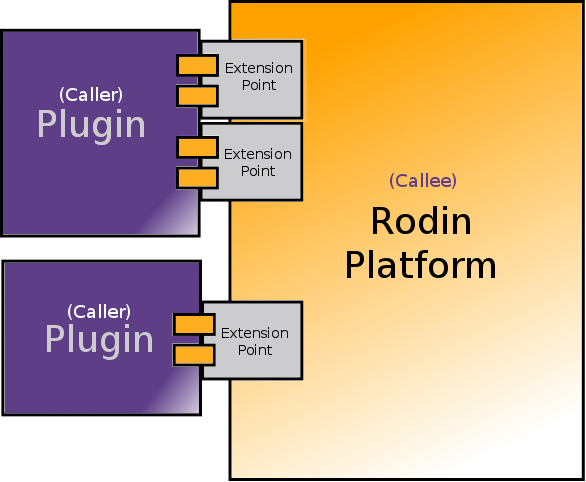
\includegraphics[scale=0.25]{Rodin.png}
\caption{Plug-ins and extension points} 
\label{Fig:Rodin Platform}
\end{figure}

In particular, it is possible to add new reasoners, which will schematically run as follows:
\begin{itemize}
\item Input: a sequent Hypotheses $\vdash$ Goal.
\item Invocation of an SMT solver.
\item Output: a proof rule.
\end{itemize}

\subsection{Integration of a SMT Solver into Rodin}
\begin{itemize}
\item A formula $A$ is \textit{valid} in a theory $T$ if $A$ evaluates to $true$ in every model $M$ of $T$.
\item A formula $A$ is \textit{satisfiable} in a theory $T$ if there is a model $M$ for $T$ in which $A$ evaluates to $true$. Otherwise, $A$ is \textit{unsatisfiable}.
\end{itemize}

It can be deduced that if a formula is unsatisfiable, its negation is valid. In other words, if $A \land \lnot B$ is unsatisfiable, then $A \limp B$ is valid. As a consequence, an Event-B sequent is not passed as is to an SMT solver, but its negation is taken as input by the SMT solver.
Conversely, if a formula is satisfiable, it means that a counter-example exists for its negation.

\begin{figure}
\centering
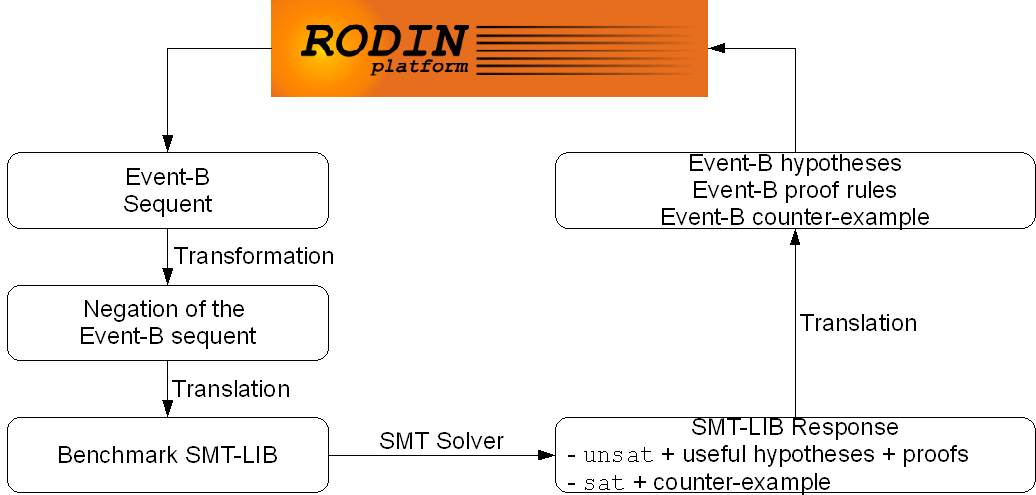
\includegraphics[scale=0.5]{Integration_SMT.png}
\caption{Integration of an SMT solver} 
\label{Fig:SMT solver}
\end{figure}

The main difficulties are all related to the translation steps. They cover several sub-tasks, such as selecting the hypotheses, choosing the SMT solver to be addressed, determining the format of the benchmark to be generated (SMT-LIB 1.2 or SMT-LIB 2.0), keeping a link between Event-B hypotheses and the associated hypotheses in SMT-LIB format...\newline


SMT plugins can be found at the following address \url{https://rodin-b-sharp.svn.sourceforge.net/svnroot/rodin-b-sharp/trunk/_exploratory/fages/}:
\begin{itemize}
\item fr.systerel.smt.provers.core divided in following packages:
	\begin{itemize}
	\item br.ufrn.smt.solver.preferences (Preference page creation in Rodin to handle solvers' configuration)
	\item br.ufrn.smt.solver.translation (Event-B Proof Obligations to SMT translation)
	\item fr.systerel.smt.provers.ast (Description of SMT language tree structure)
	\item fr.systerel.smt.provers.ast.commands (Description of SMT commands tree structure)
	\item fr.systerel.smt.provers.ast.responses (Description of SMT responses tree structure)
	\item fr.systerel.smt.provers.core (Entry point to communicate with SMT solvers) 
	\item fr.systerel.smt.provers.internal.core (The plugin core)
	\end{itemize}
\item fr.systerel.smt.provers.ui 
	\begin{itemize}
	\item fr.systerel.smt.provers.internal.ui (Entry point to communicate with Rodin platform User Interface)
	\end{itemize}
\item fr.systerel.smt.provers.tests (Tests for Event-B to SMT translation)
\end{itemize}
%% ------------------------------------------------------- %%
%% SMT-LIB 1.2
%% ------------------------------------------------------- %%
\section{From Event-B to SMT-LIB 1.2}
\subsection{From Event-B AST to SMT-LIB v1.2 AST}
The purpose of this section is to give the translation from the Event-B Abstract Syntax Tree (AST) to an SMT-LIB AST.
The \texttt{org.eventb.core.ast} plug-in for the Rodin platform allows to manipulate Event-B mathematical formulas as trees of nodes. 

The translation is expressed in a left-to-right direction, with the $\rightsquigarrow$ symbol. For example, the following conversion indicates that the
SMT-LIB syntax for the $(x < y)$ Event-B formula is $(< x~y)$:\[ (x < y) \rightsquigarrow (< x~y) \]

\paragraph{From SET to FOL}
A many-sorted formula, i.e.\ a formula containing set symbols (let's call it a SET formula), can be translated into an equivalent one belonging to first-order logic (FOL). It is enough to be convinced of such a transformation to think to the characteristic function, which takes the value 1 for elements in the set X and the value 0 for other elements. 
Note that this translation only applies to formulas based on basic sets (i.e sets that are not sets of sets), and we only refer to basic sets in the following sections. For any basic set $E$, let's introduce the unary predicate $E_x$ such that $E_x$ is true if and only if $x$ belongs to $E$.

The translation from a SET formula to a FOL formula is defined in Table \ref{SET2FOL}, where $E$ and $F$ are sets. Both formulas are expressed in Event-B language syntax. 
\begin{table}[htbp]
\begin{center}
\begin{tabular}{|c|c|}
 \hline
 \textbf{SET formula} & \textbf{FOL formula} \\ 
 \hline
 $x \in E$ & $E_x$ \\ 
 $x \notin E$ & $\neg E_x$ \\
 $E \subseteq F$ & $\forall{x}.(E_x \Rightarrow F_x)$ \\ 
 $E \nsubseteq F$ & $\exists{x}.(E_x \wedge \neg F_x)$ \\ 
 $E \subset F$ & $\forall{x}.(E_x \Rightarrow F_x) \wedge \exists{x}.(\neg E_x \wedge F_x)$ \\ 
 $E \not\subset F$ & $\forall{x}.(F_x \Rightarrow E_x) \wedge \exists{x}.(\neg F_x \wedge E_x)$ \\ 
 $E = F$ & $\forall{x}.(E_x \Longleftrightarrow F_x)$ \\ 
 $E \neq F$ & $\exists{x}.(E_x \wedge \neg F_x) \vee \exists{x}.(F_x \wedge \neg E_x)$ \\ 
 $x \in E \cap F$ & $E_x \wedge F_x$ \\ 
 $x \in E \cup F$ & $E_x \vee F_x$ \\ 
 $x \in E \setminus F$ & $E_x \wedge \neg F_x$ \\
 $x \in \{x_1, ..., x_n\}$ & $x = x_1 \vee ... \vee x = x_n$ \\
 $x \in \varnothing$ & $\perp$ \\
 $x \in x_1 .. x_n$ & $(x \geqslant x_1) \wedge (x \leqslant x_n)$ \\
 $x \in \nat$ & $x \geqslant 0$ \\
 $x \in \natn$ & $x > 0$ \\
 $x = \min(E)$ & $ E_x \wedge \forall{y}.(E_y \Rightarrow (y \geqslant x))$ \\
 $x = \max(E)$ & $ E_x \wedge \forall{y}.(E_y \Rightarrow (y \leqslant x))$ \\
 \hline
\end{tabular} 
\end{center}
\caption{From SET to FOL}
\label{SET2FOL}
\end{table}

\paragraph{From FOL to SMT-LIB}
An association between formulas in SMT-LIB format and formulas in first-order logic is given in the \S6 Semantics of the SMT-LIB specification\cite{SMTLIB06}.

\paragraph{From Event-B to SMT-LIB}
It is possible to derivate a translation from Event-B predicates to SMT-LIB formulas from the previous observations, as detailed in Table \ref{BPRED2SMTLIB}.
\begin{table}[htbp]
\begin{center}
\begin{tabular}{ccc}
 \textbf{Event-B predicate} & \textbf{$\rightsquigarrow$} & \textbf{SMT-LIB formula} \\ 
 $\top$ & & $\True$ \\
 $\bot$ & & $\False$ \\
 $P \land Q$ & & $(and~P~Q)$ \\
 $P \lor Q$ & & $(or~P~Q)$ \\
 $\lnot P$ & & $(not~P)$ \\
 $bool(P)$ & & $(ite~P~\True~\False)$ \\
 $P \limp Q$ & & $(implies~P~Q)$ \\
 $P \leqv Q$ & & $(iff~P~Q)$ \\
 $\forall{x}.(P)$ & & $(forall~(?x~Int)~P)$ \\
 $\exists{x}.(P)$ & & $(exists~(?x~Int)~P)$ \\
 $x = y$ & & $(=~x~y)$ \\
 $x \neq y$ & & $(not~(=~x~y))$ \\
 $x < y$ & & $(<~x~y)$ \\
 $x \leq y$ & & $(<=~x~y)$ \\
 $x > y$ & & $(>~x~y)$ \\
 $x \geq y$ & & $(>=~x~y)$ \\
\end{tabular} 
\end{center}
\caption{From Event-B predicates to SMT-LIB formulas}
\label{BPRED2SMTLIB}
\end{table}

In the same manner, the Event-B expressions can be transformed in SMT-LIB format (see Table \ref{BEXPR2SMTLIB}).

\begin{table}[htbp]
\begin{center}
\begin{tabular}{ccc}
 \textbf{Event-B expression} & \textbf{$\rightsquigarrow$} & \textbf{SMT-LIB formula} \\ 
 $x + y$ & & $(+~x~y)$ \\
 $x - y$ & & $(-~x~y)$ \\
 $-x$ & & $\sim x$ \\
 $x * y$ & & $(*~x~y)$ \\
 $x \div y$ & & $(/~x~y)$ \\
 $x \bmod y$ & & $(\%~x~y)$ \\
\end{tabular} 
\end{center}
\caption{From Event-B expressions to SMT-LIB formulas}
\label{BEXPR2SMTLIB}
\end{table}

\paragraph{Example}
How to translate the following formula $a \in b .. c$? 
The first step is to translate it as a FOL formula: 
$(a >= b) \wedge (a <= c)$. 
In Ints theory, where $a$ is defined as being an integer and $>=$ and $<=$ are defined as predicates of arity 2 on integers, it is possible to write the corresponding SMT-LIB formula: $(and~(>=~a~b)~(<=~a~c))$. 

\subsection{From Event-B sequents to benchmarks}
The SMT-LIB parser/checker version 3.0\cite{SMT-LIB} has been used to validate the format of the produced benchmarks.

\paragraph{Assumptions and Formulas}
It is possible to build a mapping between the sequents and the SMT-LIB benchmarks (see Figure 13 in \cite{SMTLIB06}): an hypothesis of a sequent is to be matched to a benchmark \textbf{assumption}; the goal of a sequent is to be matched to a benchmark \textbf{formula}. 

\paragraph{Typing Environment}
The typing environment is to be matched to benchmarks \textbf{extrasorts}, \textbf{extrapreds}, \textbf{extrafuns} and/or \textbf{assumption}. The following rules apply for the typing environment $\{t \mapsto T\}$, where identifier $t$ has type $T$:
\begin{itemize}
\item If $T$ is the $\intg$ predefined type of the Event-B 
mathematical language, the typing environment is represented 
with the  $:extrafuns~((t~Int))$ SMT-LIB declaration.
\item If $T$ is the $\Bool$ predefined type, it is
represented with the $:extrafuns~((t~Bool))$ declaration.
\item If $T$ is a carrier set, it is represented
with the $:extrafuns~((t~T))$ declaration.
\item If $T$ is a cartesian product of two basic types, i.e.\
$T = T_1~\cprod~T_2$, where $T_1$ and $T_2$ are basic types,
and $t~=~(t_1~\mapsto~t_2)$, it is represented with the 
$:extrafuns~((t_1~T_1)~(t_2~T_2))$ declaration.
\item If $T$ is a power-set of a basic type, i.e.\
$T~=~\pow(S)$, where $S$ is a basic type, it is represented 
with the $:extrasorts~((t) (S))$ declaration, and with an
additional assumption: $t \subseteq S$ (see the low-level
specification for the expected SMT-LIB syntax for this 
assumption).
\item If $T$ is a power-set of a cartesian product, i.e.\
$T~=~\pow(T_1~\cprod~T_2)$, where $T_1$ and $T_2$ are basic
types, it is represented with the $:extrafuns~((t~T_1~T_2))$ 
or the $:extrapreds~((t~T_1~T_2))$ declaration. The former
is used if $t$ is a function, and the latter if $t$ is a 
relation.
\end{itemize}

\paragraph{Theories}
The Ints theory, dedicated to integer numbers, and the Bools theory, dedicated to booleans, are the only applicable theories when considering mathematical  sequents based on the Event-B language. 

\paragraph{Logics}
Some sublogics of the main SMT-LIB logic (first-order logic with equality) are listed on the dedicated web page\cite{SMTLIB}.

Thus, QF\_LIA is for example the logic for quantifier-free linear integer arithmetic (i.e.\ boolean combinations of inequations between linear polynomials over integer variables). It refers to the Ints theory.

The linear\_order\_int and linear\_arith theories described in the taxonomy\cite{TAXO09} are to be matched to this logic. 

\paragraph{Example}
For example, if the goal for a sequent is $0 < n + 1$, under the hypothesis $n \in \nat$, in the $\{n \mapsto \intg\}$ typing environment, the associated benchmark is structured as detailed below:
\begin{align*}
(benchmark~&example.smt                      \\
           &:status~sat                      \\
           &:logic~QF\_LIA                   \\
           &:extrafuns~((n~Int))             \\
           &:assumption~(>=~n~0)             \\
           &:formula~(<~0~(+~n~1))) 
\end{align*}

\subsection{Targeted SMT Solvers}
The following SMT solvers, which support the SMT-LIB 1.2 format, have been used via the SMT plugin in the Rodin platform: 
\begin{itemize}
\item VeriT\cite{VERIT} (VeriT takes part of DECERT program and provides the possibility to use an extended SMT-Lib format).
\item Alt-Ergo\cite{ALTERGO} (Alt-Ergo takes part of DECERT program and is known to have good results with arithmetics formulas).
\item CVC3\cite{CVC3} (CVC3 si known to support many logics and is available easily for linux or windows platforms).
\item Z3\cite{Z3} (Z3 is updated regularly and available on windows platforms).
\end{itemize}

\paragraph{}
To implement the transformation from Event-B sequents to SMT-LIB benchmarks, and in particular the SET to FOL translation, we have first used the extensions to the SMT-LIB library implemented in the veriT solver, namely macro definitions and lambda expressions (see \cite{BSMT10}). However, if the targeted solver is not veriT, it is necessary to convert the Event-B sequents from the extended SMT-LIB format to the standard SMT-LIB format (see \cite{RODINSMT10}), using the $-print-simp-and-exit$ option provided by veriT.
In order to simplify the processing sequence, we now rely on the translator provided by the Predicate Prover available in Rodin (see $trunk/RodinCore/org.eventb.pptrans$, among the sources\cite{SOURCES} of the Rodin platform). 
Concerning arithmetics, we have continued from the prototype\cite{B2SMT09} implemented last year.

NB: Relations and functions are not yet fully handled and will be tackled in year 3.

%% ------------------------------------------------------- %%
%% SMT-LIB 2.0                                             
%% ------------------------------------------------------- %%
\section{SMT-LIB 2.0}
\subsection{SMT-LIB 2.0 vs SMT-LIB 1.2}
The steps engaged to set up Version 2.0 have consisted in setting up a concrete syntax which is simpler and leaner than Version 1.2.
The two major additions are the following:
\begin{itemize}
\item A mechanism that approximates parametric sorts and polymorphic function symbols in theory declarations.
\item A command language :
\begin{itemize}
\item to allow user asserting and retracting formulas incrementally,
\item to define new sort and function symbols
\item to check the satisfiability of the asserted formulas and query their found model or unsatisfiable core.
\end{itemize}
\end{itemize}


\begin{figure}
\centering
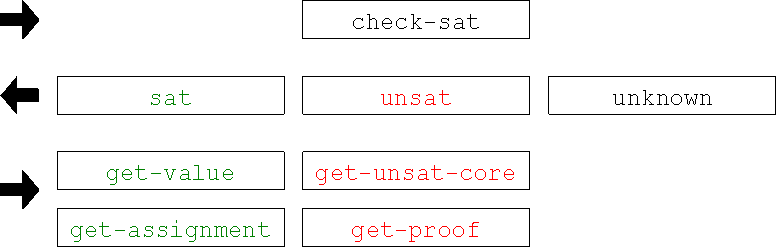
\includegraphics[scale=0.5]{SMT20.png}
\caption{SMT-LIB 2.0 Script Commands} 
\label{Fig:SMT-LIB 2.0}
\end{figure}

\subsection{Solvers' Proof Format}
The commands \textit{get-model} and \textit{get-proof} introduced in SMT-lib v2.0 will be interesting to expose model or counterexample in Rodin. But nowadays, the proof format has not been defined yet in the SMT-Lib v2.0. The Deliverable 7 of DECERT (Task 4:Preliminary Report on a Generic Proof Format for SMT Solvers) will make it clearer and so the integration in Rodin will be possible. 
 
\section{From Event-B to SMT-LIB 2.0}

\subsection{From Event-B AST to SMT-LIB v2.0 AST}
The translation from the Event-B Abstract Syntax Tree (AST) to an SMT-LIB AST V2.0 is very similar to the one to SMT-LIB v1.2 and will not defined again.

\subsection{From Event-B sequents to benchmarks}
The SMT-LIB parser/checker version 3.0 (\url{http://www.cs.uiowa.edu/~astump/software/ocaml-smt2.zip}) has been used to validate the format of the produced benchmarks.

\paragraph{Assertion}
There is no longer \textbf{assumption} and \textbf{formula} to refer to hypotheses and goal of a sequent. Each hypothesis or goal can be mapped with a benchmark \textbf{assert}. 

\paragraph{Typing Environment}
The typing environment is to be matched to benchmarks \textbf{declare-sort},  \textbf{declare-fun} and/or \textbf{assert}. The following rules apply for the typing environment $\{t \mapsto T\}$, where identifier $t$ has type $T$:
\begin{itemize}
\item If $T$ is the $\intg$ predefined type of the Event-B 
mathematical language, the typing environment is represented 
with the $(declare-fun~t~()~Int)$  SMT-LIB declaration.
\item If $T$ is the $\Bool$ predefined type, it is
represented with the $(declare-fun~t~()~Bool)$  declaration.
\item If $T$ is a user-defined basic type, it is represented
with the $(declare-fun~t~()~T)$ declaration.
\item If $T$ is a cartesian product of two basic types, i.e.\
$T = T_1~\cprod~T_2$, where $T_1$ and $T_2$ are basic types,
and $t~=~(t_1~\mapsto~t_2)$, it is represented with the 
$(declare-fun~t~(T2)~T1)$ declaration.
%% 
%%\item If $T$ is a power-set of a basic type, i.e.\
%%$T~=~\pow(S)$, where $S$ is a basic type, it is represented 
%%with the $(declare-fun~t~()~S)$ declaration, !BEGIN TODO and with an
%%additional assumption: $t \subseteq S$ (see the low-level
%%specification for the expected SMT-LIB syntax for this 
%%assumption) !END TODO.
%%\item If $T$ is a power-set of a cartesian product, i.e.\
%%$T~=~\pow(T_1~\cprod~T_2)$, where $T_1$ and $T_2$ are basic
%%types, it is represented with the !BEGIN TODO $:extrafuns~((t~T_1~T_2))$ 
%%or the $:extrapreds~((t~T_1~T_2))$ declaration. The former
%%is used if $t$ is a function, and the latter if $t$ is a 
%%relation !END TODO.
\end{itemize}

Thus, QF\_LIA is for example the logic for unquantified integer linear arithmetic (i.e.\ boolean combinations of inequations between linear polynomials over integer variables). It refers to the Ints theory.

The linear\_order\_int and linear\_arith theories described in the taxonomy\cite{TAXO09} are to be matched to this logic. 

\paragraph{Example}
For example, if the goal for a sequent is $0 < n + 1$, under the hypothesis $n \in \nat$, in the $\{n \mapsto \intg\}$ typing environment, the associated benchmark is structured as detailed below:
\begin{align*}           
&(set-logic~QF\_LIA)                     \\
&(declare-fun~n~()~Int)                 \\
&(assert~(>=~n~0))						\\
&(assert~(not (< 0~(+~n~1))))			\\
&(check-sat)
\end{align*}


\subsection{Targeted SMT solvers}
For the moment, not every SMT solver supports SMT-Lib 2.0. During the SMT-COMP 2010, many solvers have been introduced to confront each other with SMT v2.0 benchmarks (\url{http://www.smtexec.org/exec/competitors2010.php}). Some of them only parse the 2.0 language and do not include every SMT-Lib 2.0 requirements. Here is an outlook of interesting solvers regarding SMT-lib 2.0:

\begin{itemize}
\item CVC3 \cite{CVC3}(during SMT competition, CVC3 was candidate in those following logics :$UFLRA$, $QF\_UF$, $QF\_RDL$, $QF\_IDL$, $QF\_BV$, $QF\_UFIDL$, $QF\_AX$, $AUFLIA+p$, $AUFLIA-p$, $AUFLIRA$, $QF\_AUFLIA$, $QF\_UFLRA$, $QF\_UFLIA$, $QF\_LRA$, $AUFNIRA$, $UFNIA$, $UFNIA+p$, $QF\_LIA$, $QF\_NIA$, $QF\_UFNRA$, $QF\_NRA$, $QF\_ABV$). 

\item MathSAT 5 \cite{MATHSAT} (during SMT competition, MathSAT was candidate in those following logics : $QF\_UF$, $QF\_UFLRA$, $QF\_UFLIA$, $QF\_LRA$, $QF\_LIA$).

\item OpenSmt \cite{OPENSMT}(during SMT competition, OpenSmt was candidate in those following logics : $QF\_UF$, $QF\_RDL$, $QF\_IDL$, $QF\_UFIDL$, $QF\_LRA$).

\item VeriT\cite{VERIT} (during SMT competition, VeriT was candidate in those following logics : $QF\_UF$, $QF\_RDL$, $QF\_IDL$, $QF\_UFIDL$).

\item Z3 \cite{Z3} (does not take part in SMT competition). 

\end{itemize}

These solvers parse SMT-Lib 2.0 but not do not support in general unsat core or model generation yet. Only Z3 offers an unsatisfiable core generation via the smt command \textit{(get-unsat-core)}.
%% ------------------------------------------------------- %%
%% Filtering
%% ------------------------------------------------------- %%
\section{Filtering Mechanism}
Faire reference ici aux resultats des benchmarks.
Ceux-ci doivent permettre de determiner comment maximiser les chances de reponse des solveurs SMT :
\begin{itemize}
\item Quel solveur privilegier (selon theories supportees, version SMT-LIB, etc) ?
\item Quelles options / parametres ?
\item Quelles theories ?
\item Quelles hypotheses ?
\end{itemize}

\subsection{}

\paragraph{}





%% ----------------------------- %%
%% Conclusion %%
%% ----------------------------- %%
\section{Conclusion}

\paragraph{Future work.} 

\paragraph{Acknoledgements.} 
The author thanks David D\'eharbe and V\'itor Alc\^antara de Almeida (Universidade Federal do Rio Grande do Norte, Natal, RN, Brazil), whose work on integrating SMT solvers in Rodin \cite{RODINSMT10} has provided a solid basis and has largely contributed to the contents of this deliverable.

%% ----------------------------- %%
%% Index and references
%% ----------------------------- %%
\nocite{*}
\bibliographystyle{plain}
\bibliography{biblio}

%% ----------------------------- %%
%% Index and references
%% ----------------------------- %%
\appendix
\makeatletter
\def\@seccntformat#1{Appendix~\csname the#1\endcsname:\quad}
\makeatother
\section{Benchmarking Procedure and Results}
\label{Bench}

     
\end{document}
